\section{Langkah-Langkah Percobaan}
\begin{enumerate}
    \item Kabel LAN dihubungkan dari laptop ke router, dan router ke router.
    \item Login menggunakan MAC address, lalu router direset terlebih dahulu menggunakan Winbox.
    \begin{figure}[H]
        \centering
        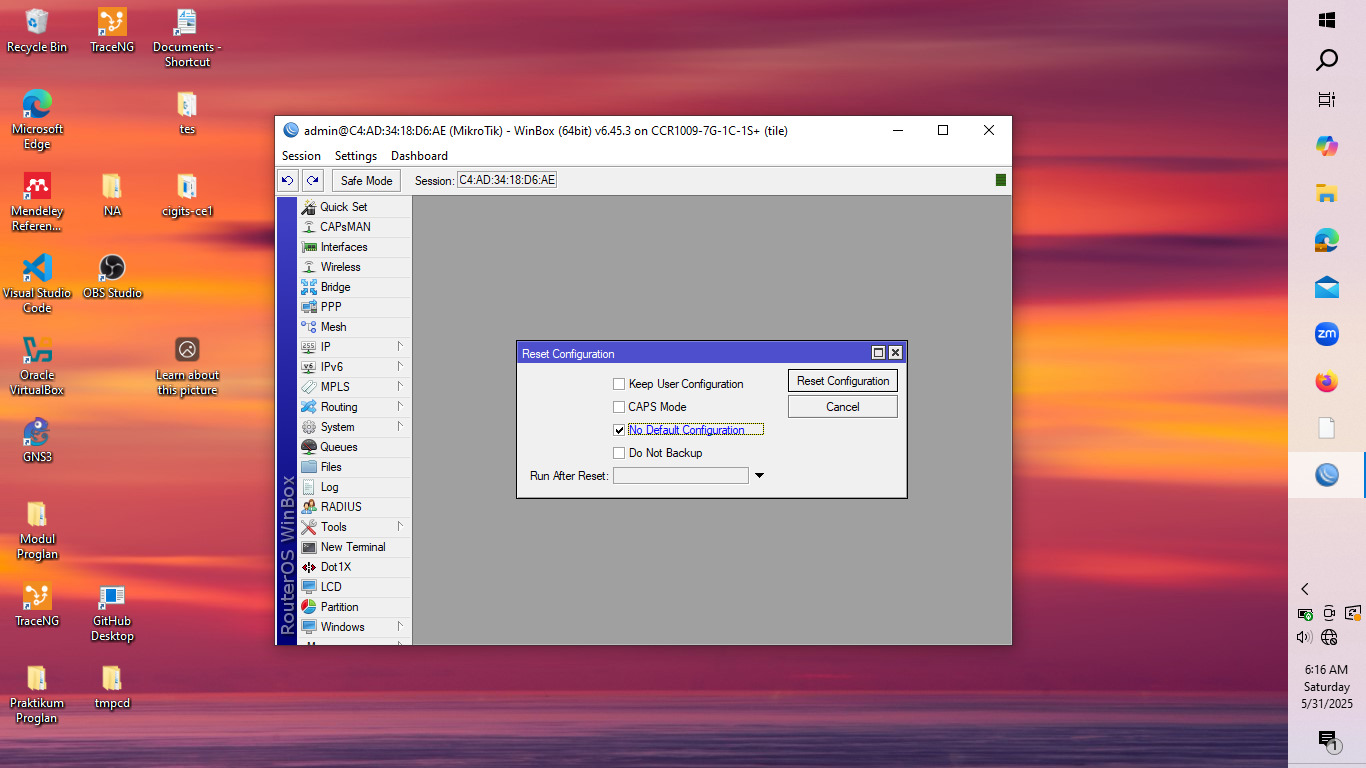
\includegraphics[width=0.5\linewidth]{gambar1.jpeg}
        \caption{Mereset Router pada Winbox}
        \label{fig:reset-router}
    \end{figure}
    \item Konfigurasi DHCP Client pada Router A
    \begin{figure}[H]
        \centering
        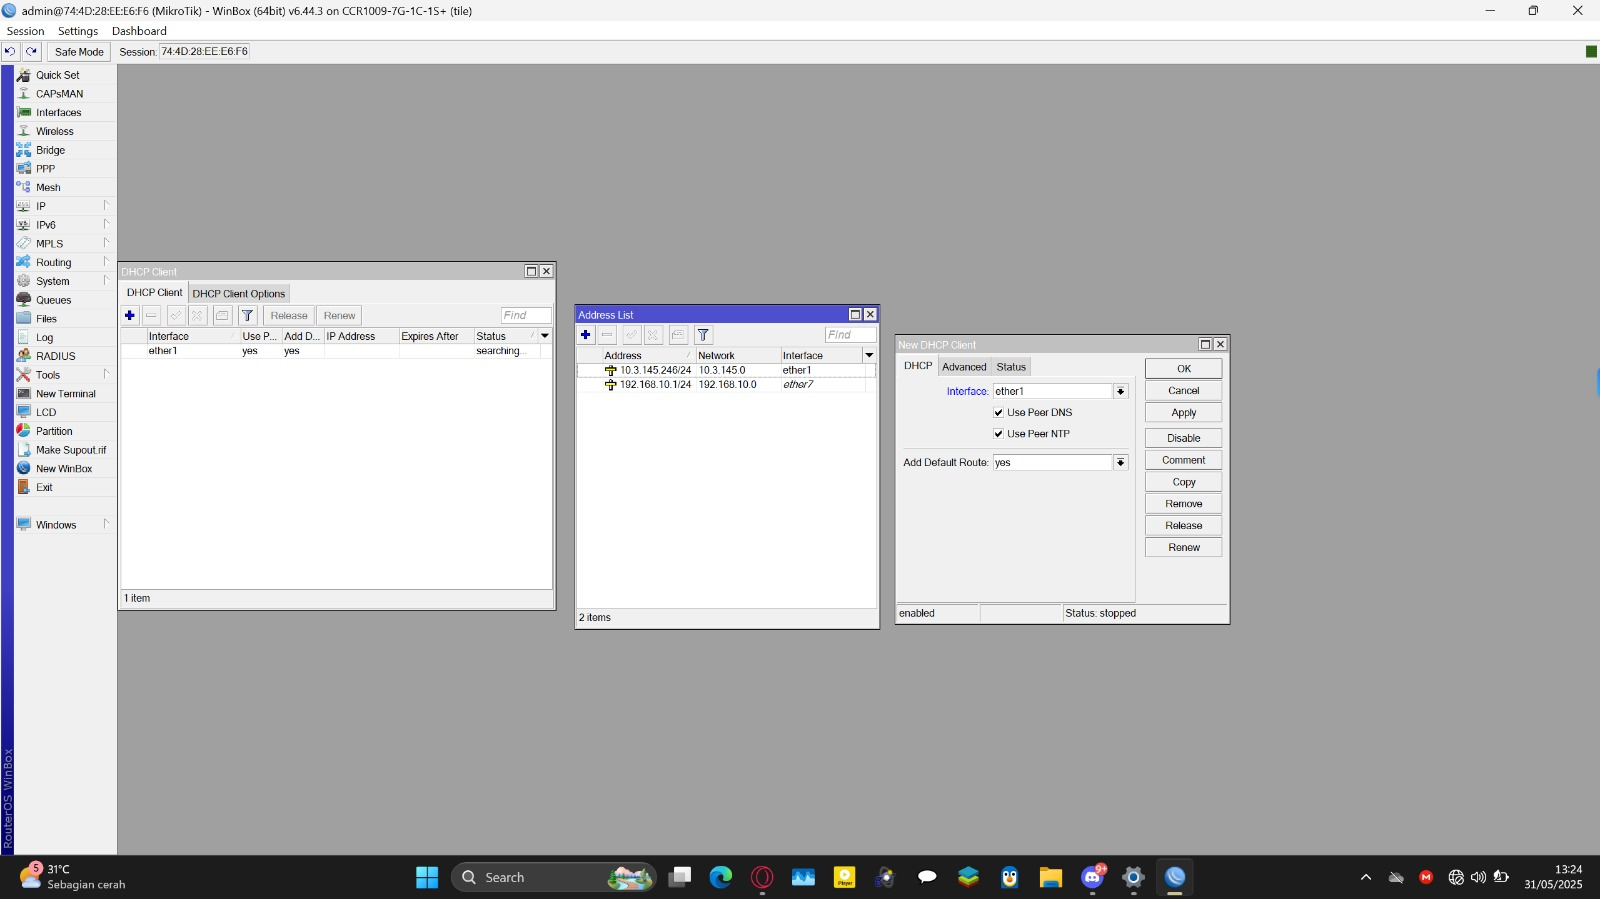
\includegraphics[width=0.5\linewidth]{gambar2.jpeg}
        \caption{Mengkonfigurasi DHCP Client pada Router A}
        \label{fig:DHCP-router-A}
    \end{figure}
    \item Menambahkan Alamat IP pada ether 7
    \begin{figure}[H]
        \centering
        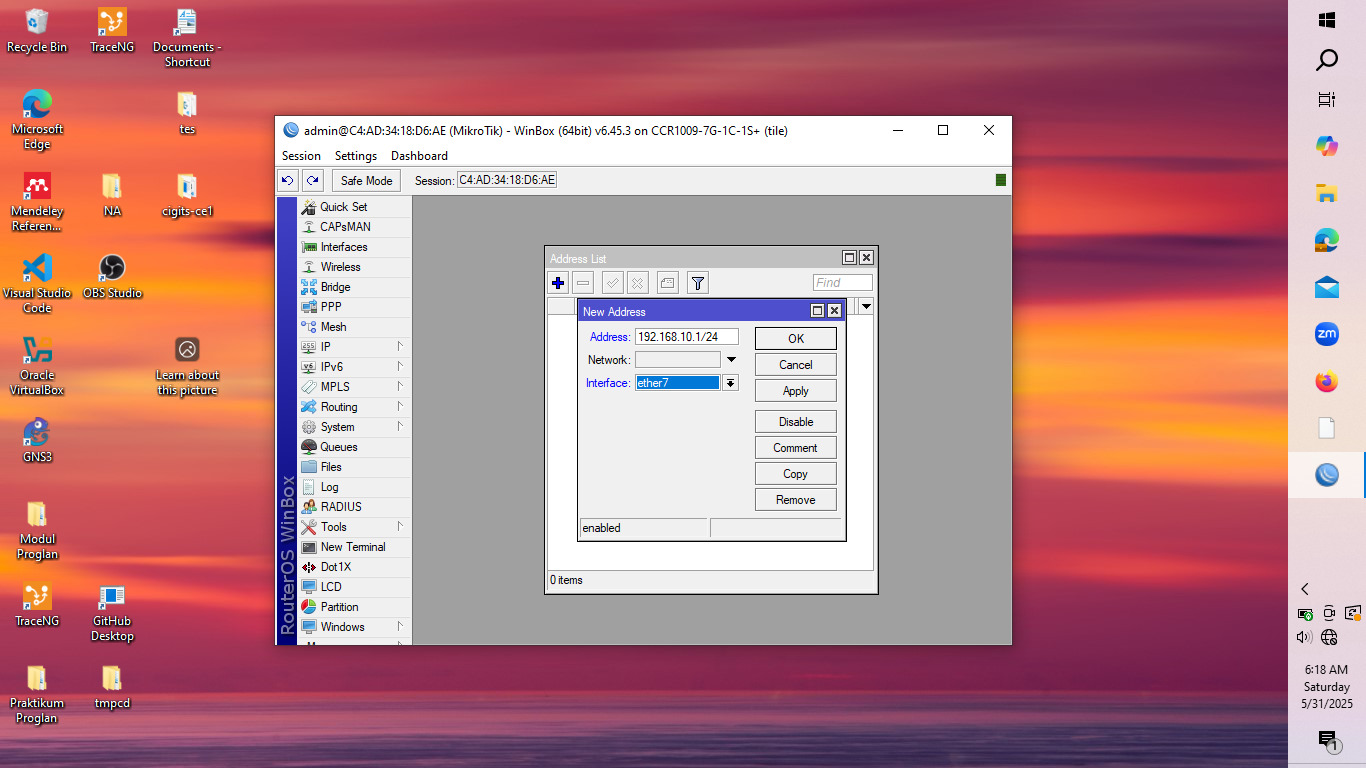
\includegraphics[width=0.5\linewidth]{gambar3.jpeg}
        \caption{Menambahkan Alamat IP pada ether 7}
        \label{fig:menambahkan-ip-ether7}
    \end{figure}
    \item Konfigurasikan DHCP server pada mikrotik
     \begin{figure}[H]
        \centering
        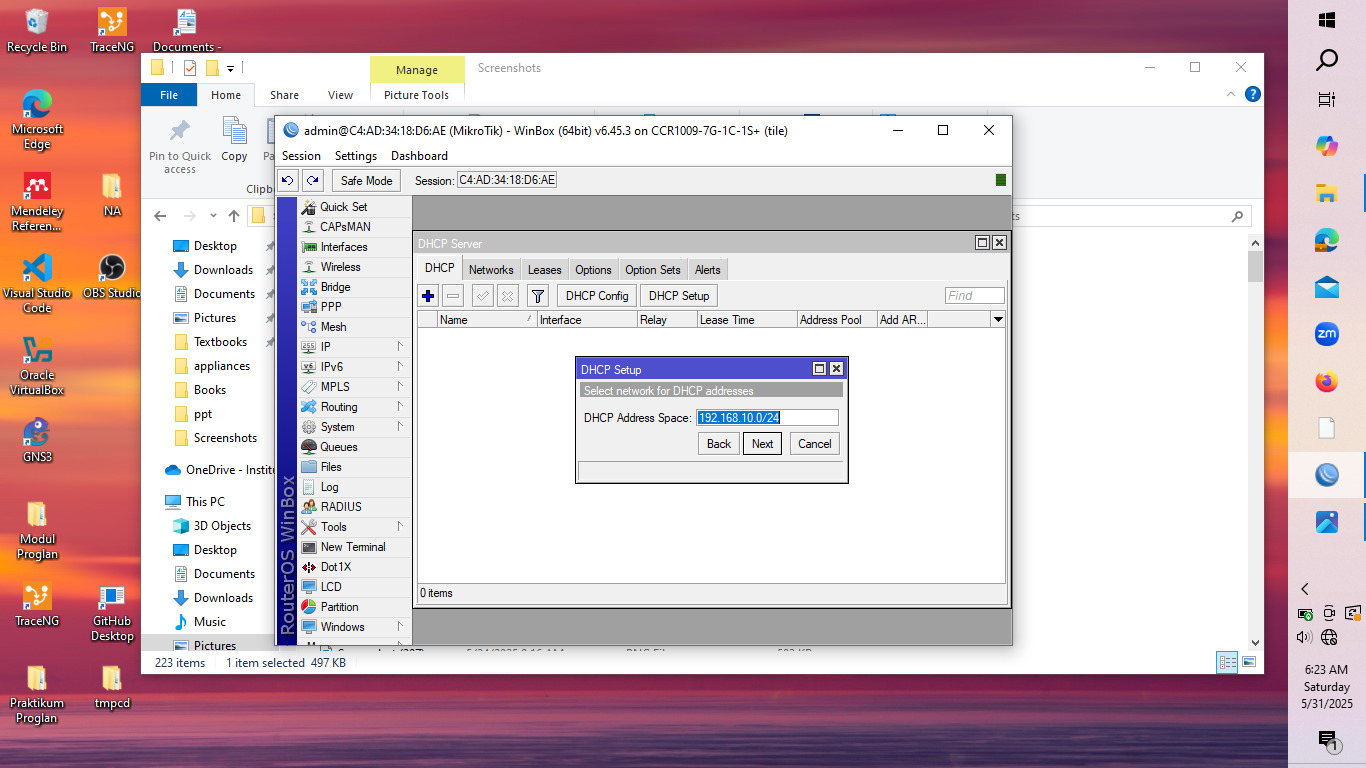
\includegraphics[width=0.5\linewidth]{gambar4a.jpeg}
        \caption{Mengkonfigurasikan DHCP server pada mikrotik}
        \label{fig:mengkonfigurasikan-dhcp-server-mikrotik}
    \end{figure}

    \begin{figure}[H]
        \centering
        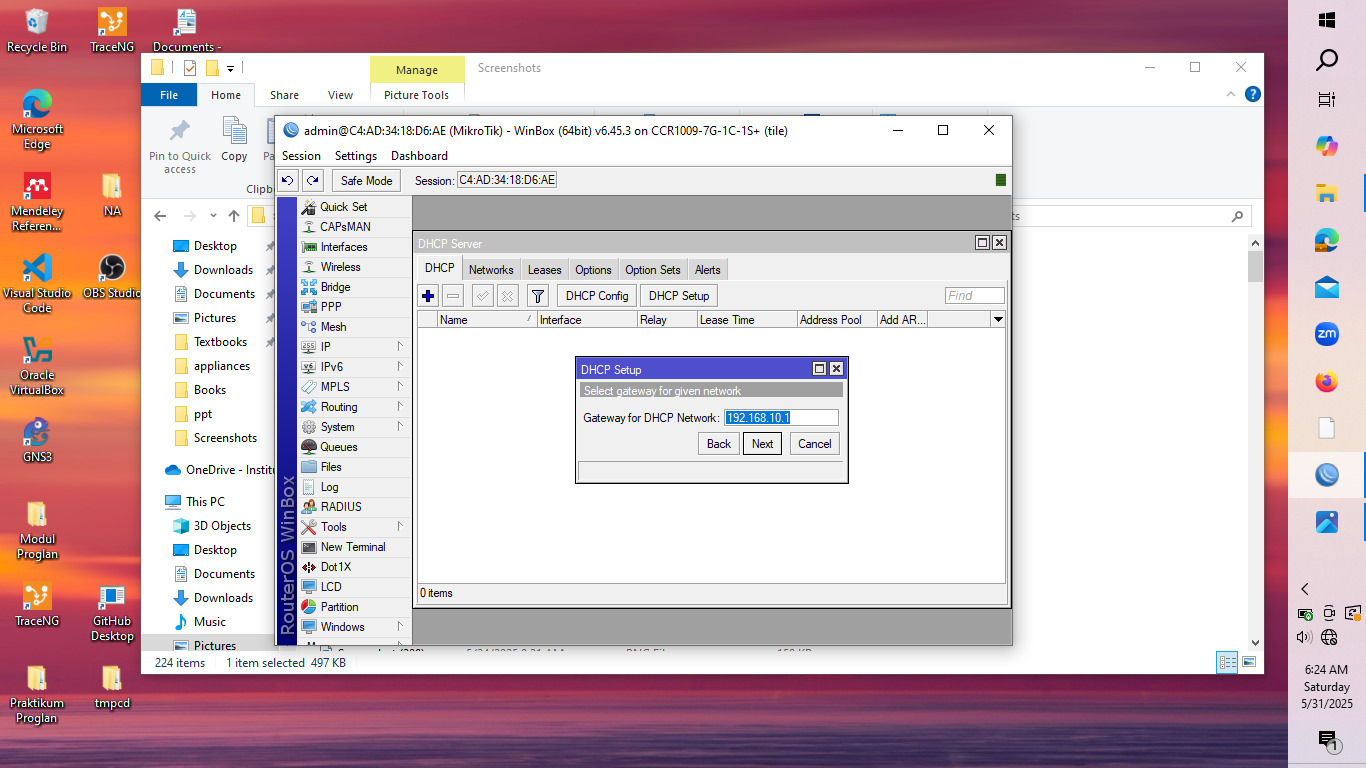
\includegraphics[width=0.5\linewidth]{gambar4b.jpeg}
        \caption{Mengkonfigurasikan DHCP server pada mikrotik}
        \label{fig:mengkonfigurasikan-dhcp-server-mikrotik}
    \end{figure}

    \begin{figure}[H]
        \centering
        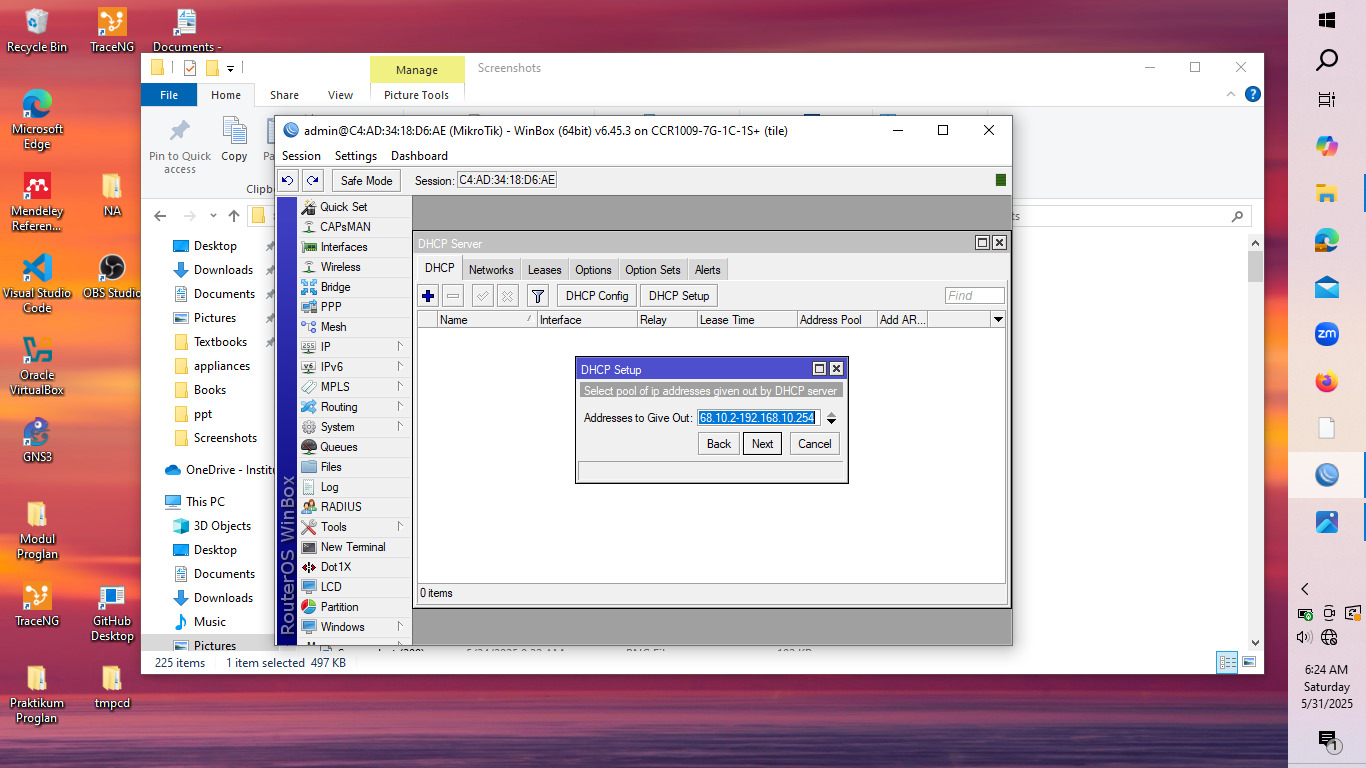
\includegraphics[width=0.5\linewidth]{gambar4c.jpeg}
        \caption{Mengkonfigurasikan DHCP server pada mikrotik}
        \label{fig:mengkonfigurasikan-dhcp-server-mikrotik}
    \end{figure}
    
    \begin{figure}[H]
        \centering
        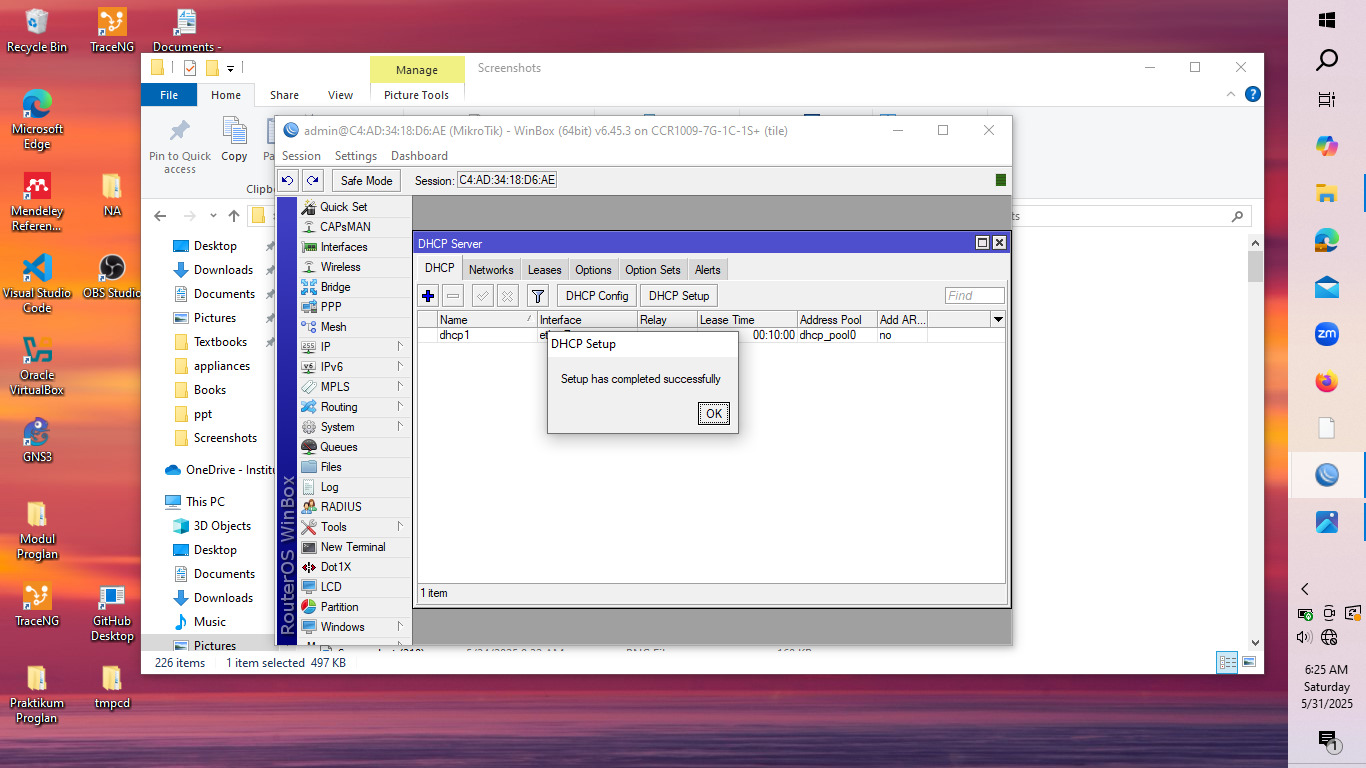
\includegraphics[width=0.5\linewidth]{gambar4d.jpeg}
        \caption{Mengkonfigurasikan DHCP server pada mikrotik}
        \label{fig:mengkonfigurasikan-dhcp-server-mikrotik}
    \end{figure}
    
    \item Konfigurasikan NAT
    \begin{figure}[H]
        \centering
        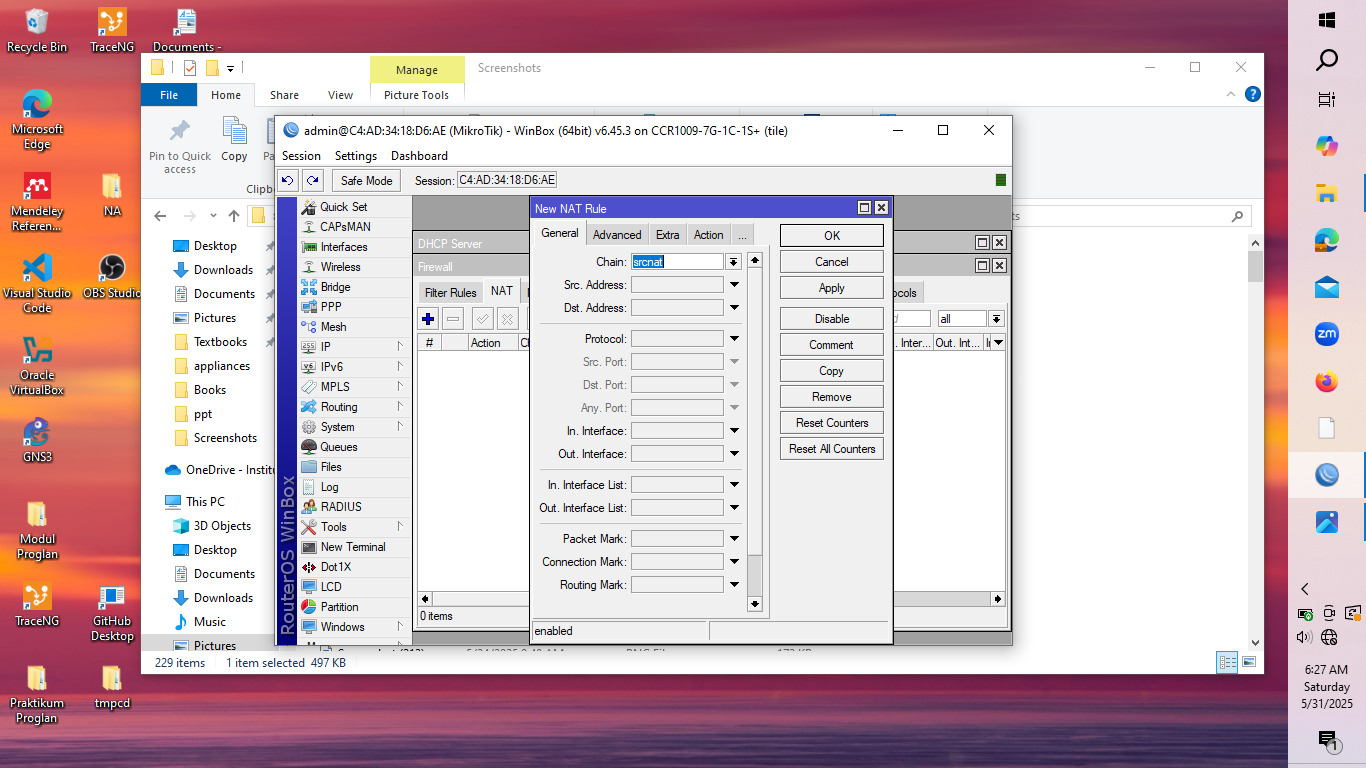
\includegraphics[width=0.5\linewidth]{gambar5a.jpeg}
        \caption{Mengkonfigurasikan NAT}
        \label{fig:mengkonfigurasikan-NAT}
    \end{figure}

    \begin{figure}[H]
        \centering
        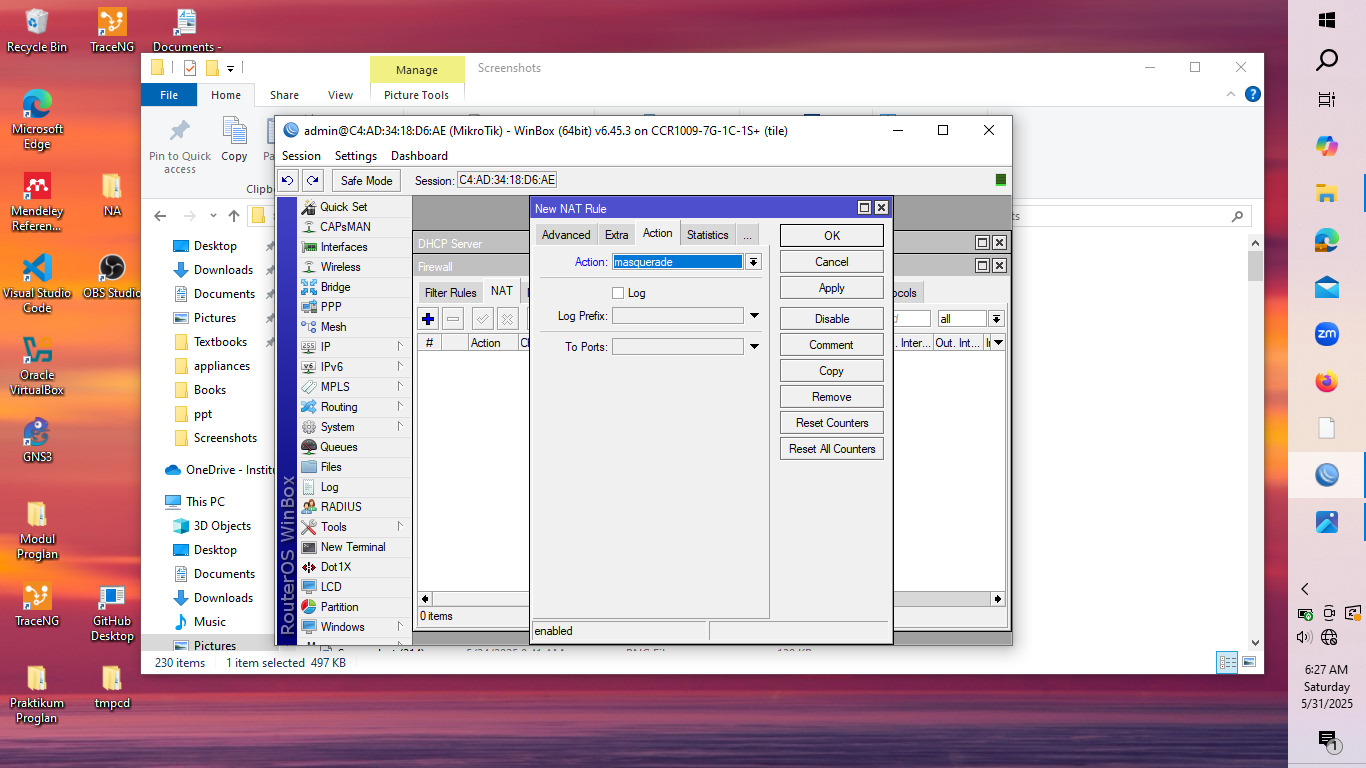
\includegraphics[width=0.5\linewidth]{gambar5b.jpeg}
        \caption{Mengkonfigurasikan NAT}
        \label{fig:mengkonfigurasikan-NAT}
    \end{figure}
    \item Lalu firewall diatur
    \begin{figure}[H]
        \centering
        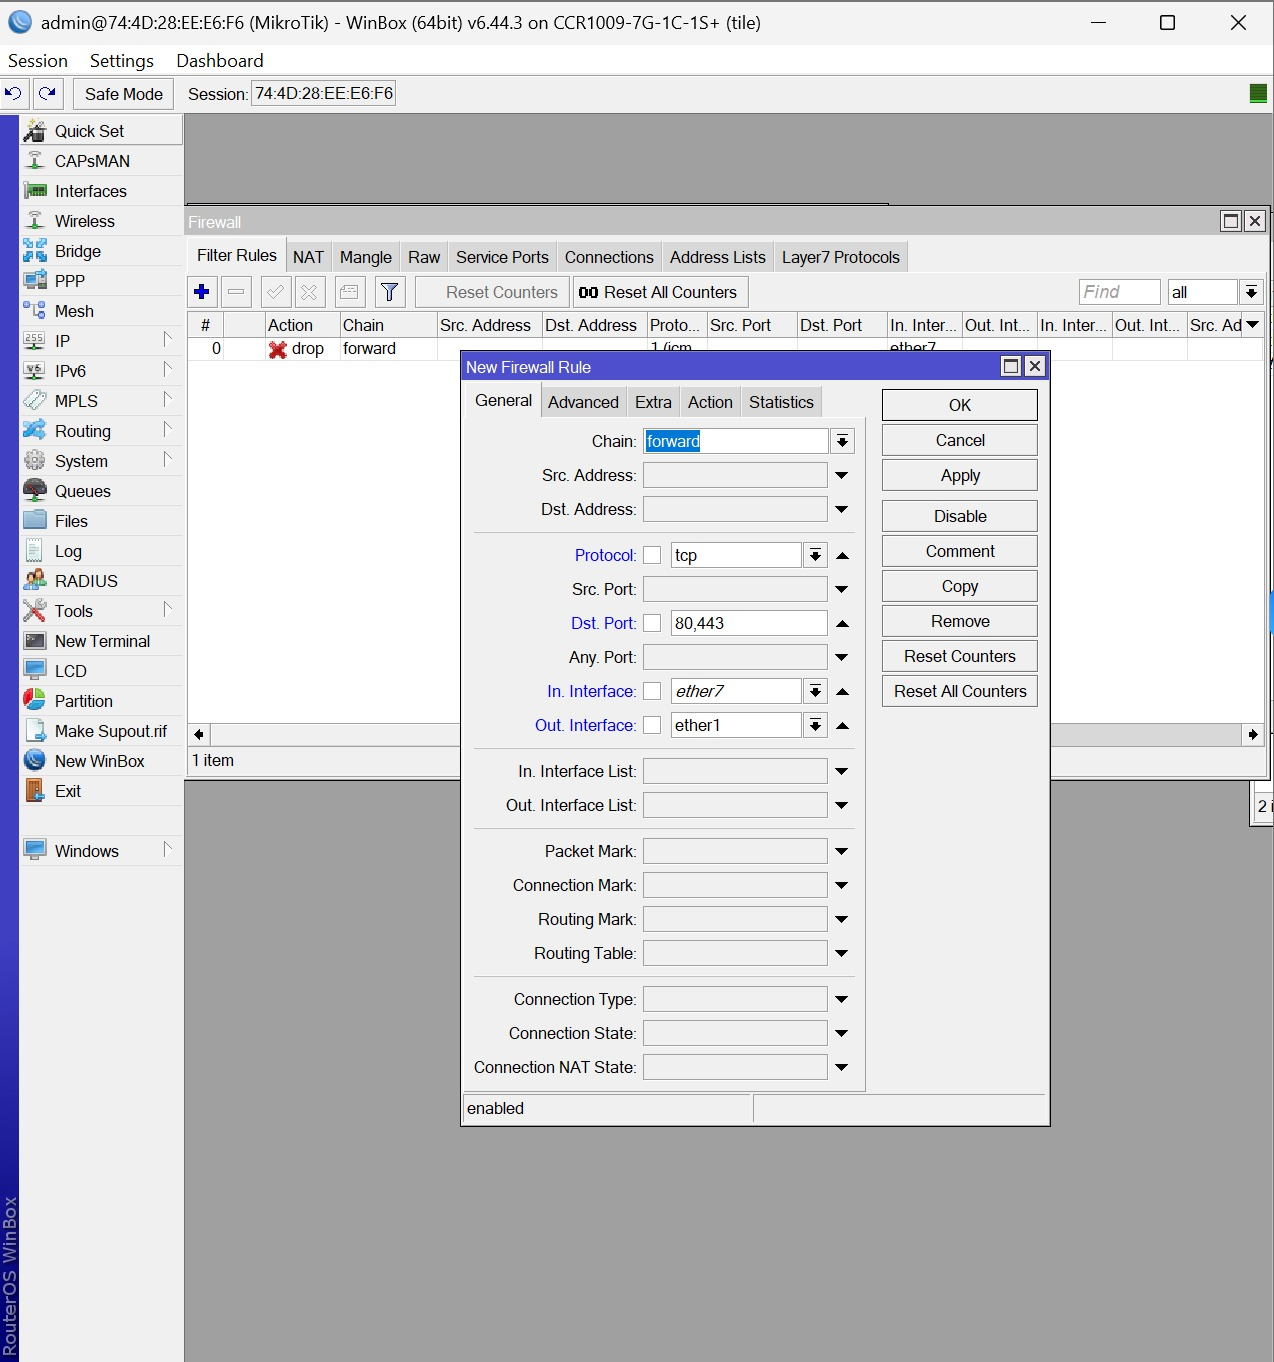
\includegraphics[width=0.5\linewidth]{gambar6.jpeg}
        \caption{Mengkonfigurasikan Firewall}
        \label{fig:mengkonfigurasikan-firewall}
    \end{figure}
    \item Mengkofigurasi Bridge pada router B 
    \begin{figure}[H]
        \centering
        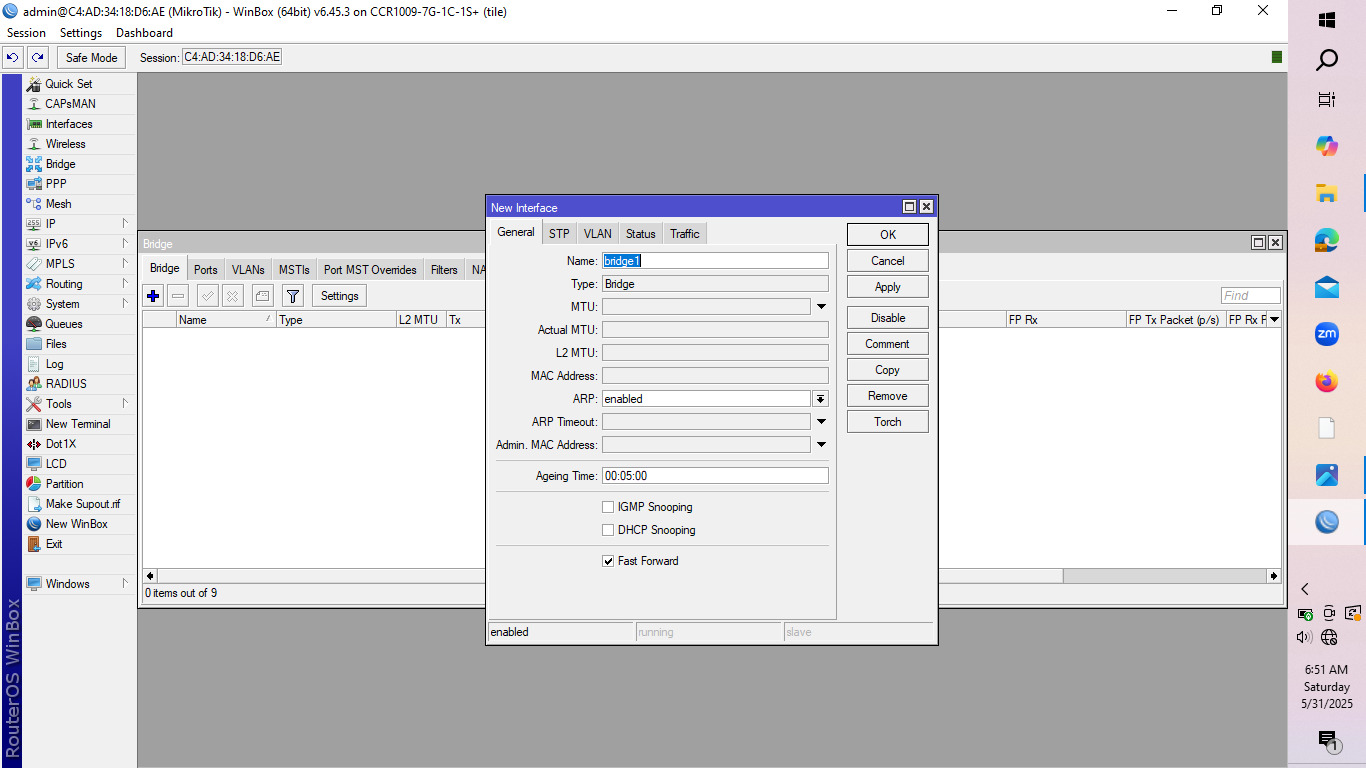
\includegraphics[width=0.5\linewidth]{gambar7a.jpeg}
        \caption{Mengkonfigurasikan Bridge pada Router B}
        \label{fig:mengkonfigurasikan-bridge-router-B}
    \end{figure}

    \begin{figure}[H]
        \centering
        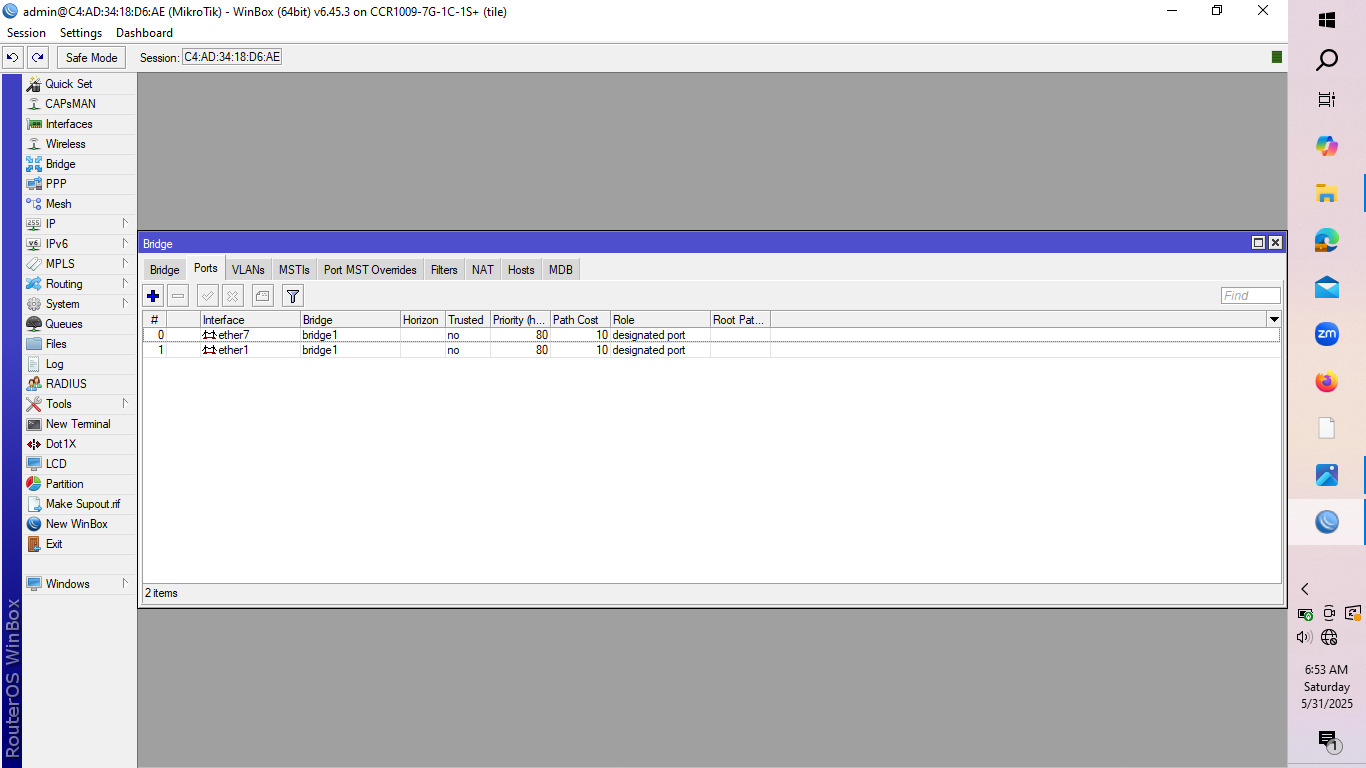
\includegraphics[width=0.5\linewidth]{gambar7b.jpeg}
        \caption{Mengkonfigurasikan Bridge pada Router B}
        \label{fig:mengkonfigurasikan-bridge-router-B}  
    \end{figure}
    \item Alamat IP dikonfigurasikan pada command prompt
    \begin{figure}[H]
        \centering
        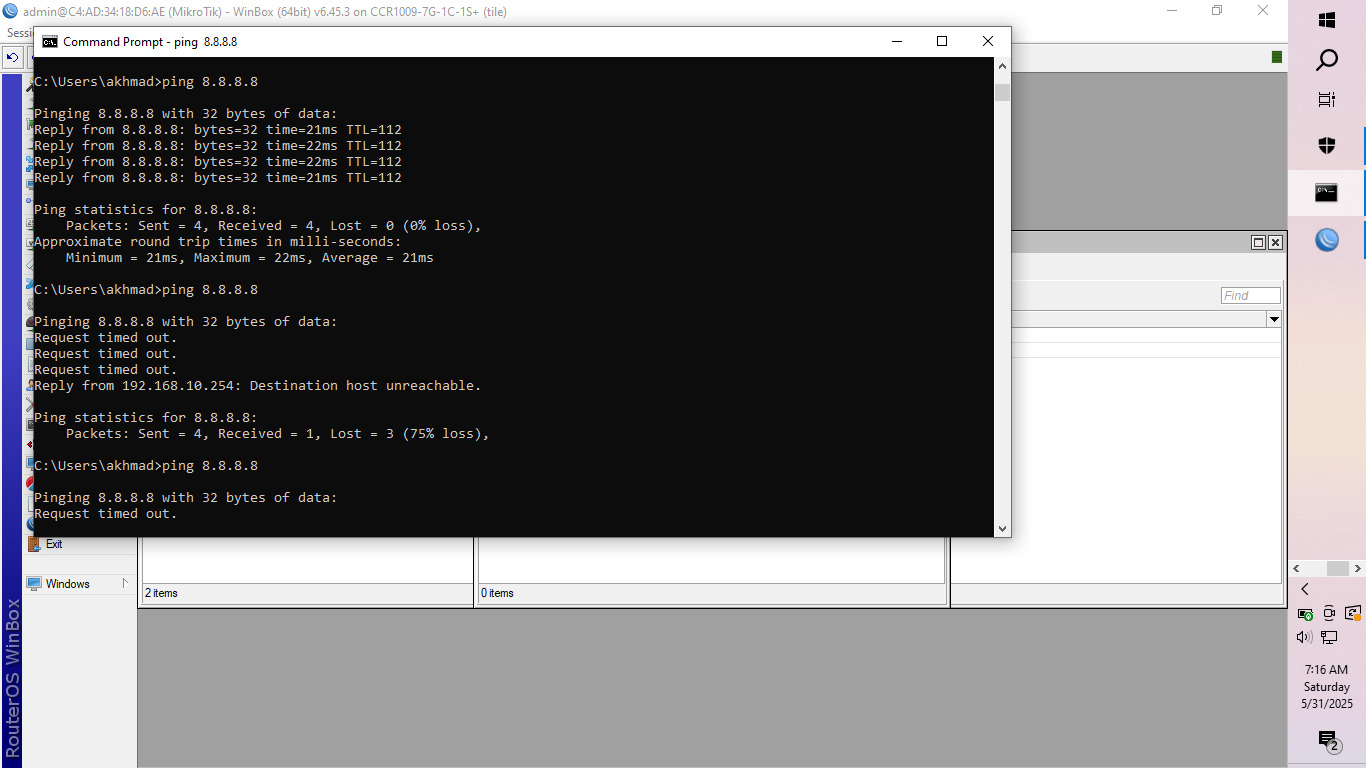
\includegraphics[width=0.5\linewidth]{gambar8a.jpeg}
        \caption{Ping dengan Firewall Aktif}
        \label{fig:ping-saat-firewall-aktif}
    \end{figure}

    \begin{figure}[H]
        \centering
        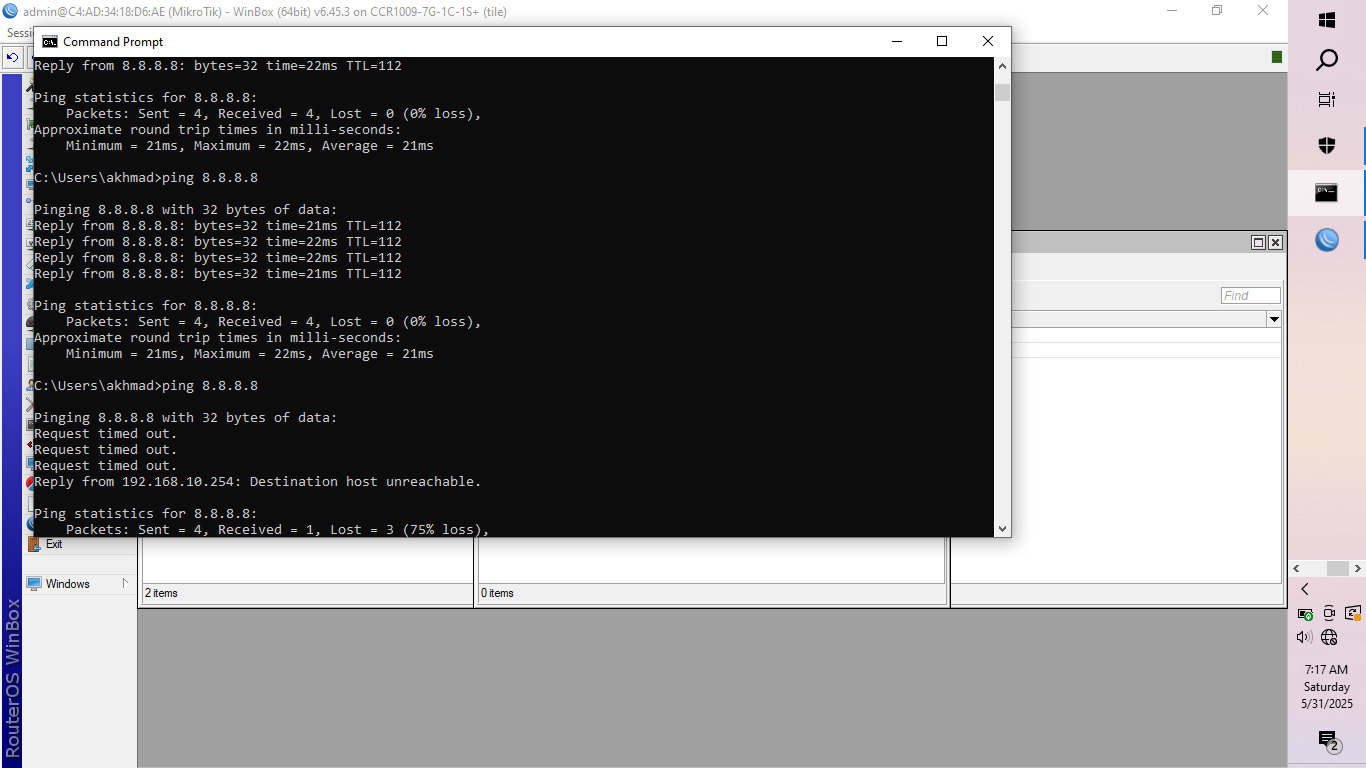
\includegraphics[width=0.5\linewidth]{gambar8b.jpeg}
        \caption{Ping dengan Firewall Tidak Aktif}
        \label{fig:ping-saat-firewall-tidak-aktif}
    \end{figure}

    

    
    

\end{enumerate}

\section{Analisis Hasil Percobaan}
Setelah melakukan percobaan, didapatkan hasil firewall yang aktif dan tidak aktif. Saat firewall aktif dan ditambahkan rule tertentu, 
ping tidak dapat dilakukan, sedangkan saat firewall tidak aktif, ping dapat dilakukan. Hal ini menunjukkan 
bahwa firewall berfungsi untuk mengatur lalu lintas jaringan dan melindungi jaringan dari akses yang tidak diinginkan.

NAT pada praktikum ini juga dilakukan dan didapatkan hasil NAT (Network Address Translation) berfungsi untuk mengubah alamat IP dari paket data yang melewati router,
sehingga memungkinkan beberapa perangkat di jaringan lokal untuk berbagi satu alamat IP publik, sehingga dapat
menghemat penggunaan alamat IP publik. Hal ini tidak hanya menghemat penggunaan alamat IP publik, tetapi juga 
memberikan lapisan tambahan dalam keamanan karena perangkat internal tidak langsung terekspos ke '
jaringan publik.



\section{Hasil Tugas Modul}
    \begin{figure}[H]
        \centering
        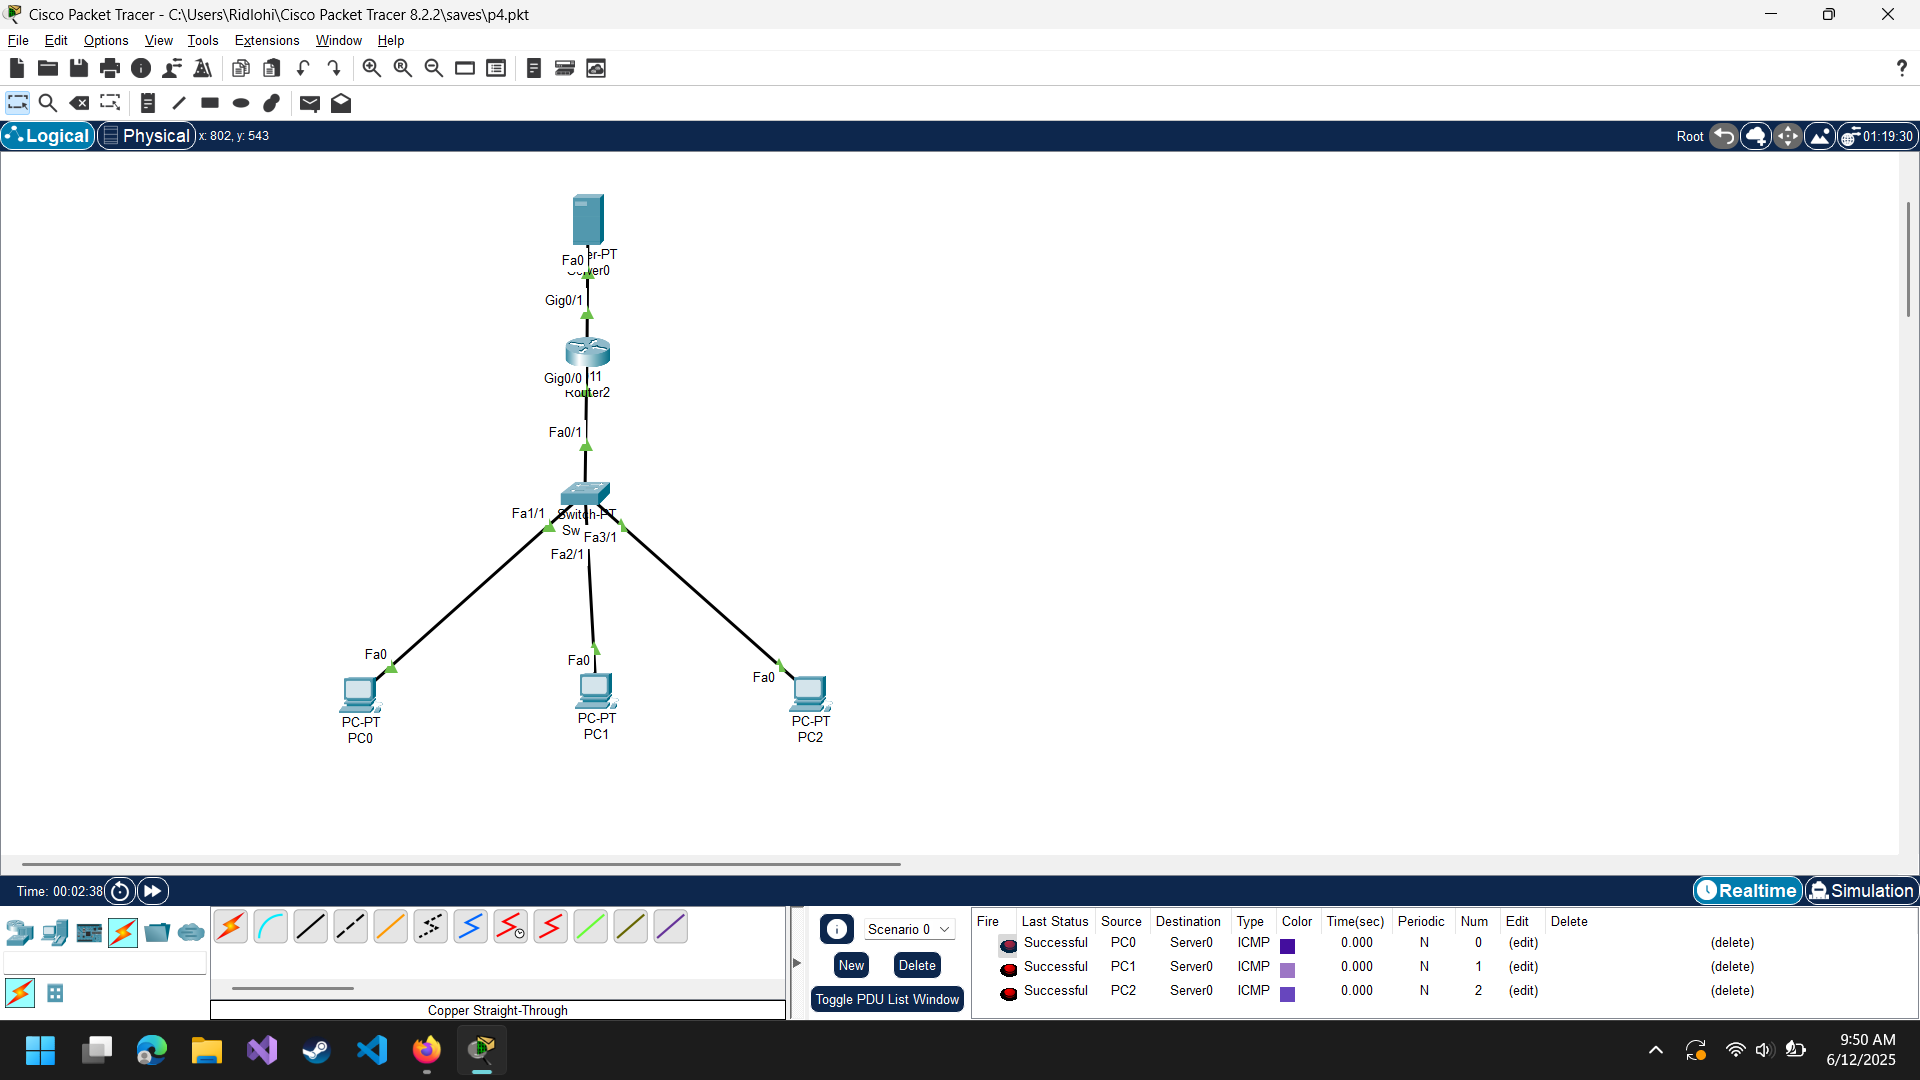
\includegraphics[width=0.5\linewidth]{pingsemuakeserver.png}
        \caption{Ping semua PC ke server}
        \label{fig:gambar}
    \end{figure}

    \begin{figure}[H]
        \centering
        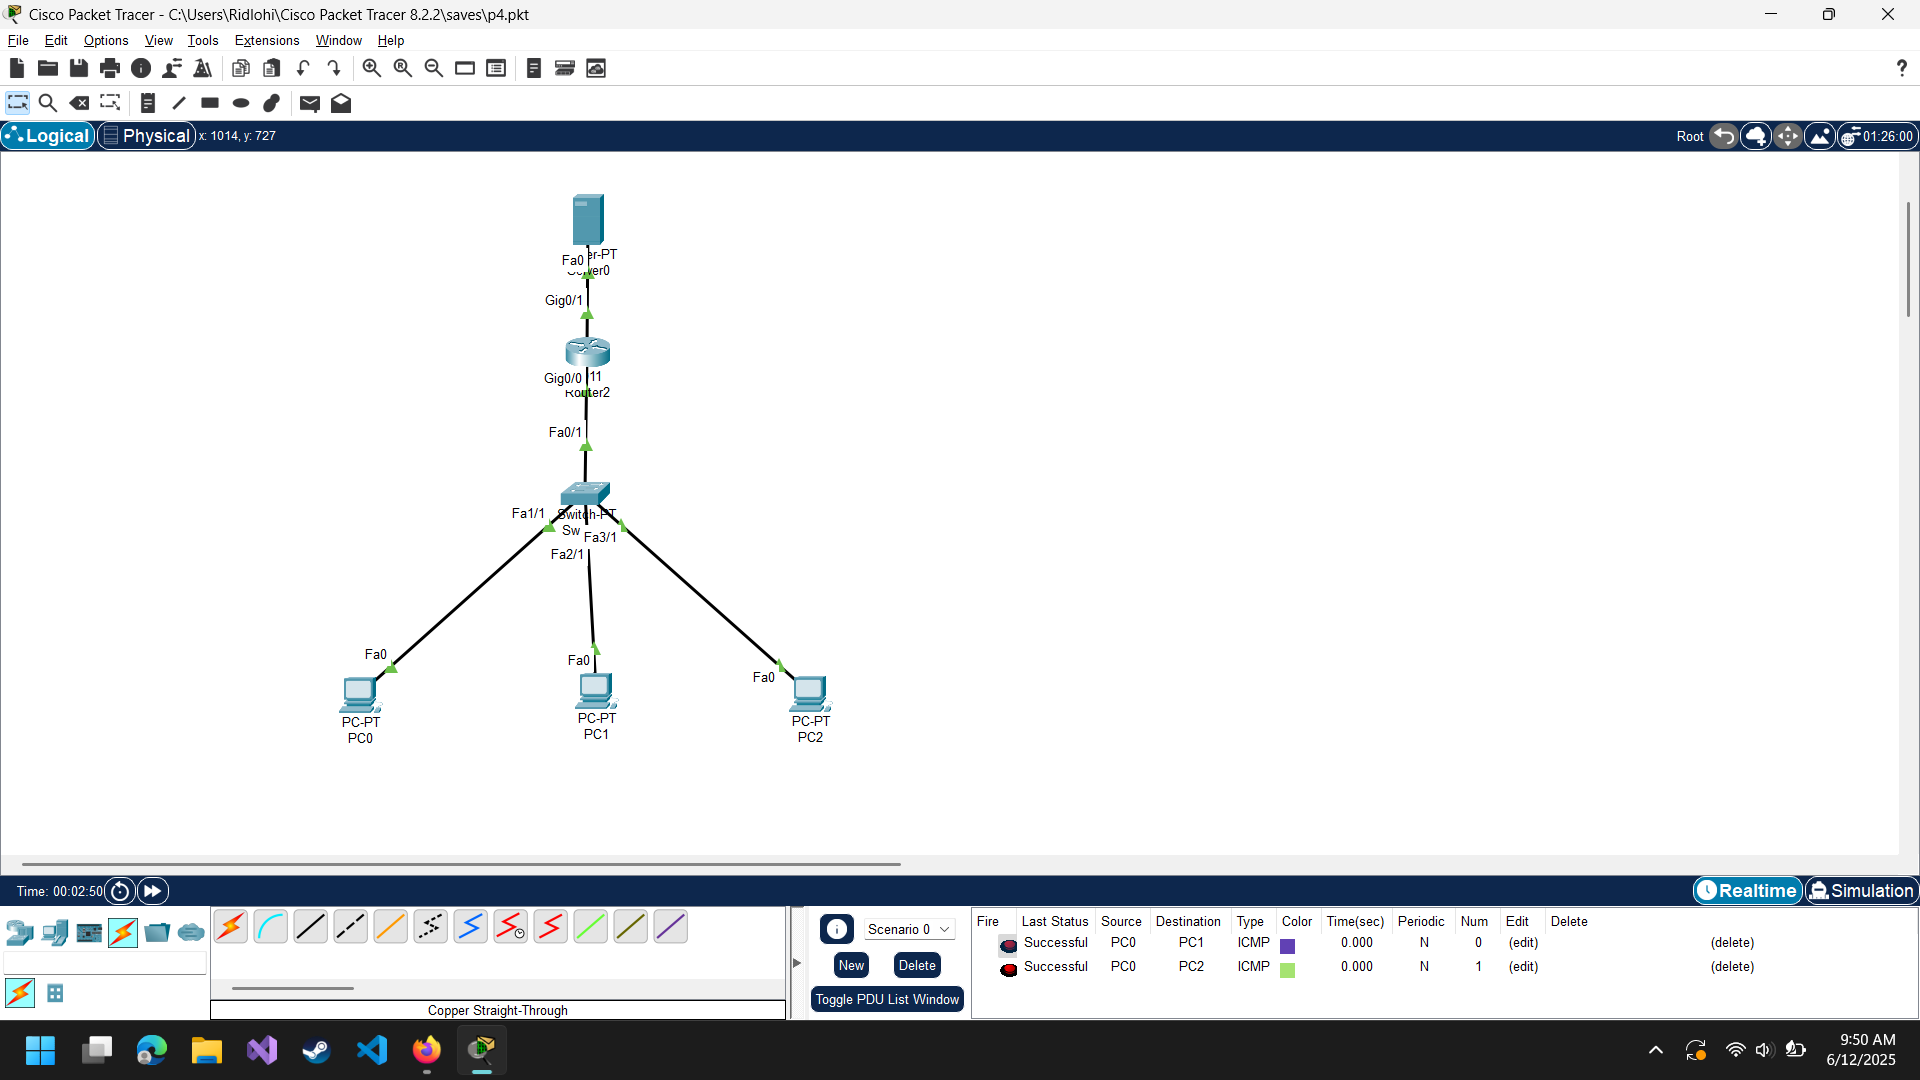
\includegraphics[width=0.5\linewidth]{pingpckepc.png}
        \caption{Ping semua PC ke PC}
        \label{fig:gambar}
    \end{figure}

    \begin{figure}[H]
        \centering
        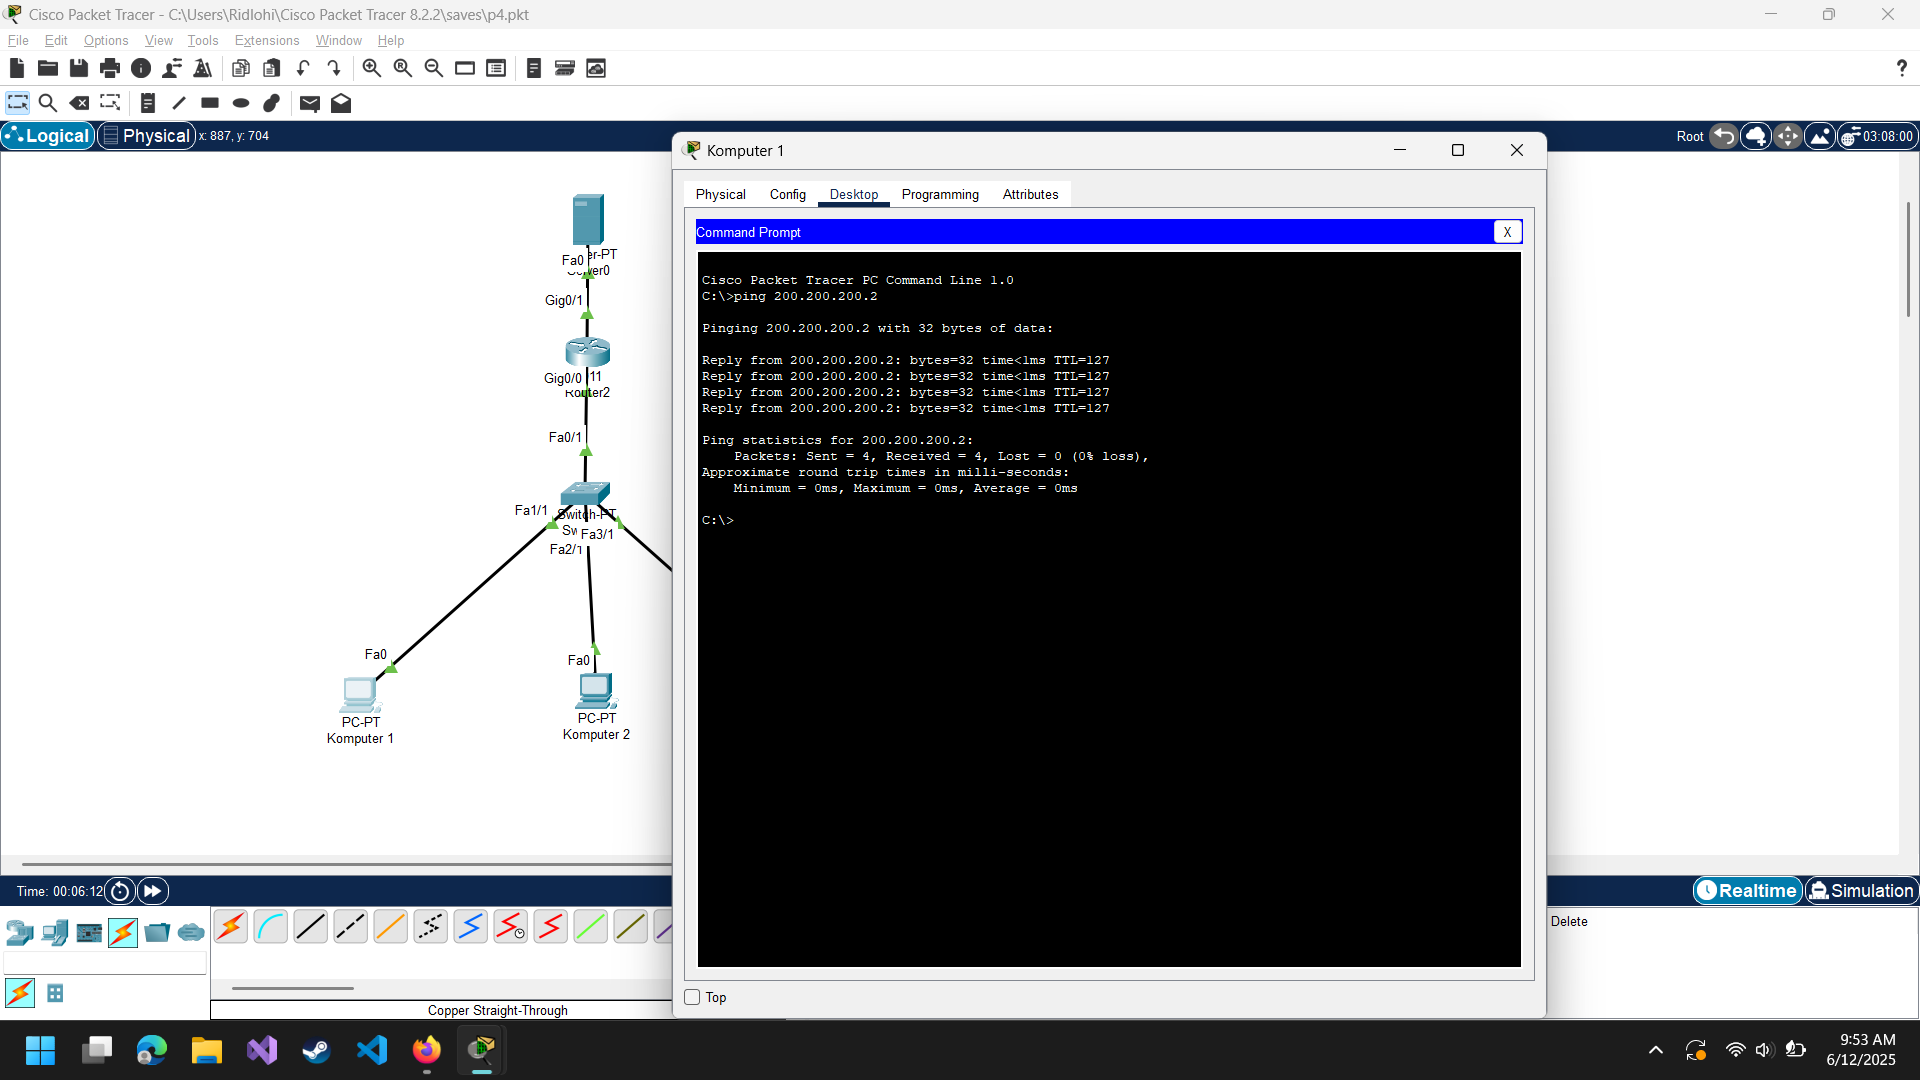
\includegraphics[width=0.5\linewidth]{pingpc1keserver.png}
        \caption{Ping PC 1 ke server}
        \label{fig:gambar}
    \end{figure}

    \begin{figure}[H]
        \centering
        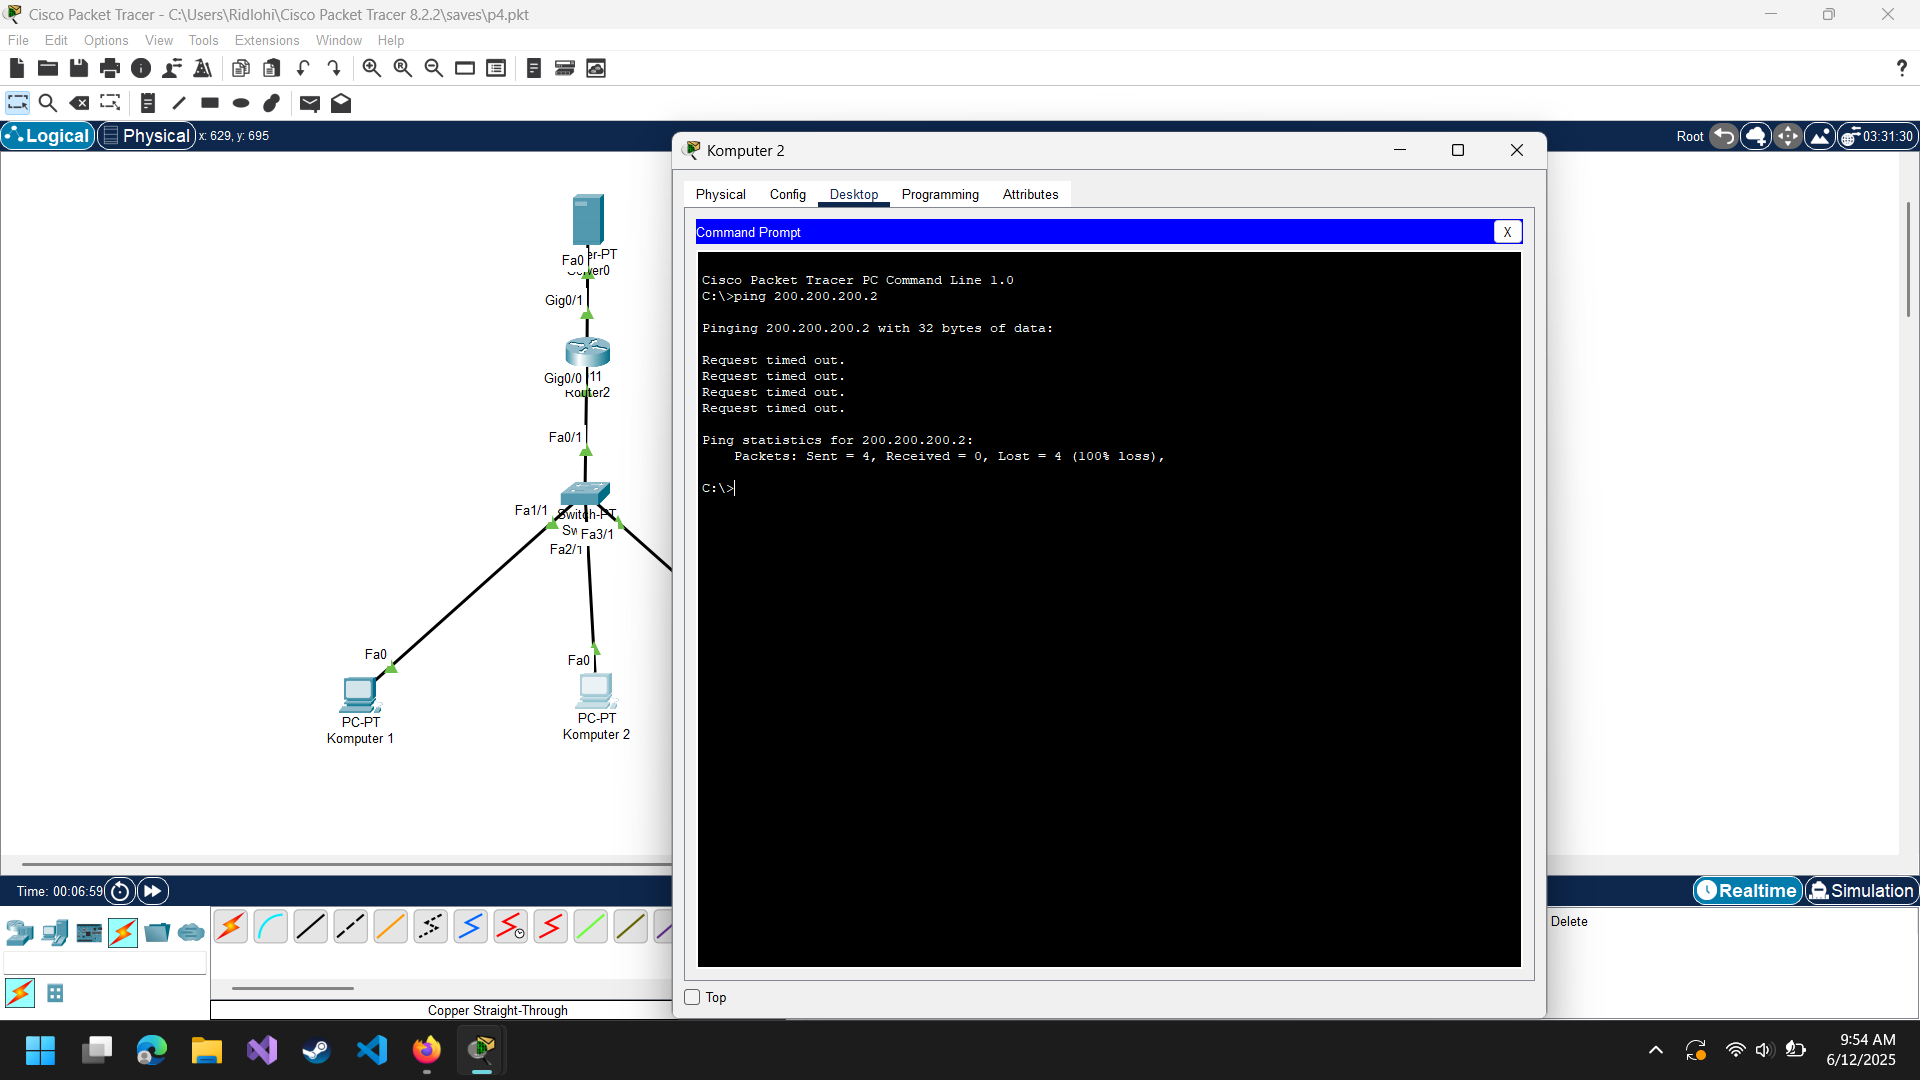
\includegraphics[width=0.5\linewidth]{pingpc2keserver.png}
        \caption{Ping PC 2 ke server}
        \label{fig:gambar}
    \end{figure}

    \begin{figure}[H]
        \centering
        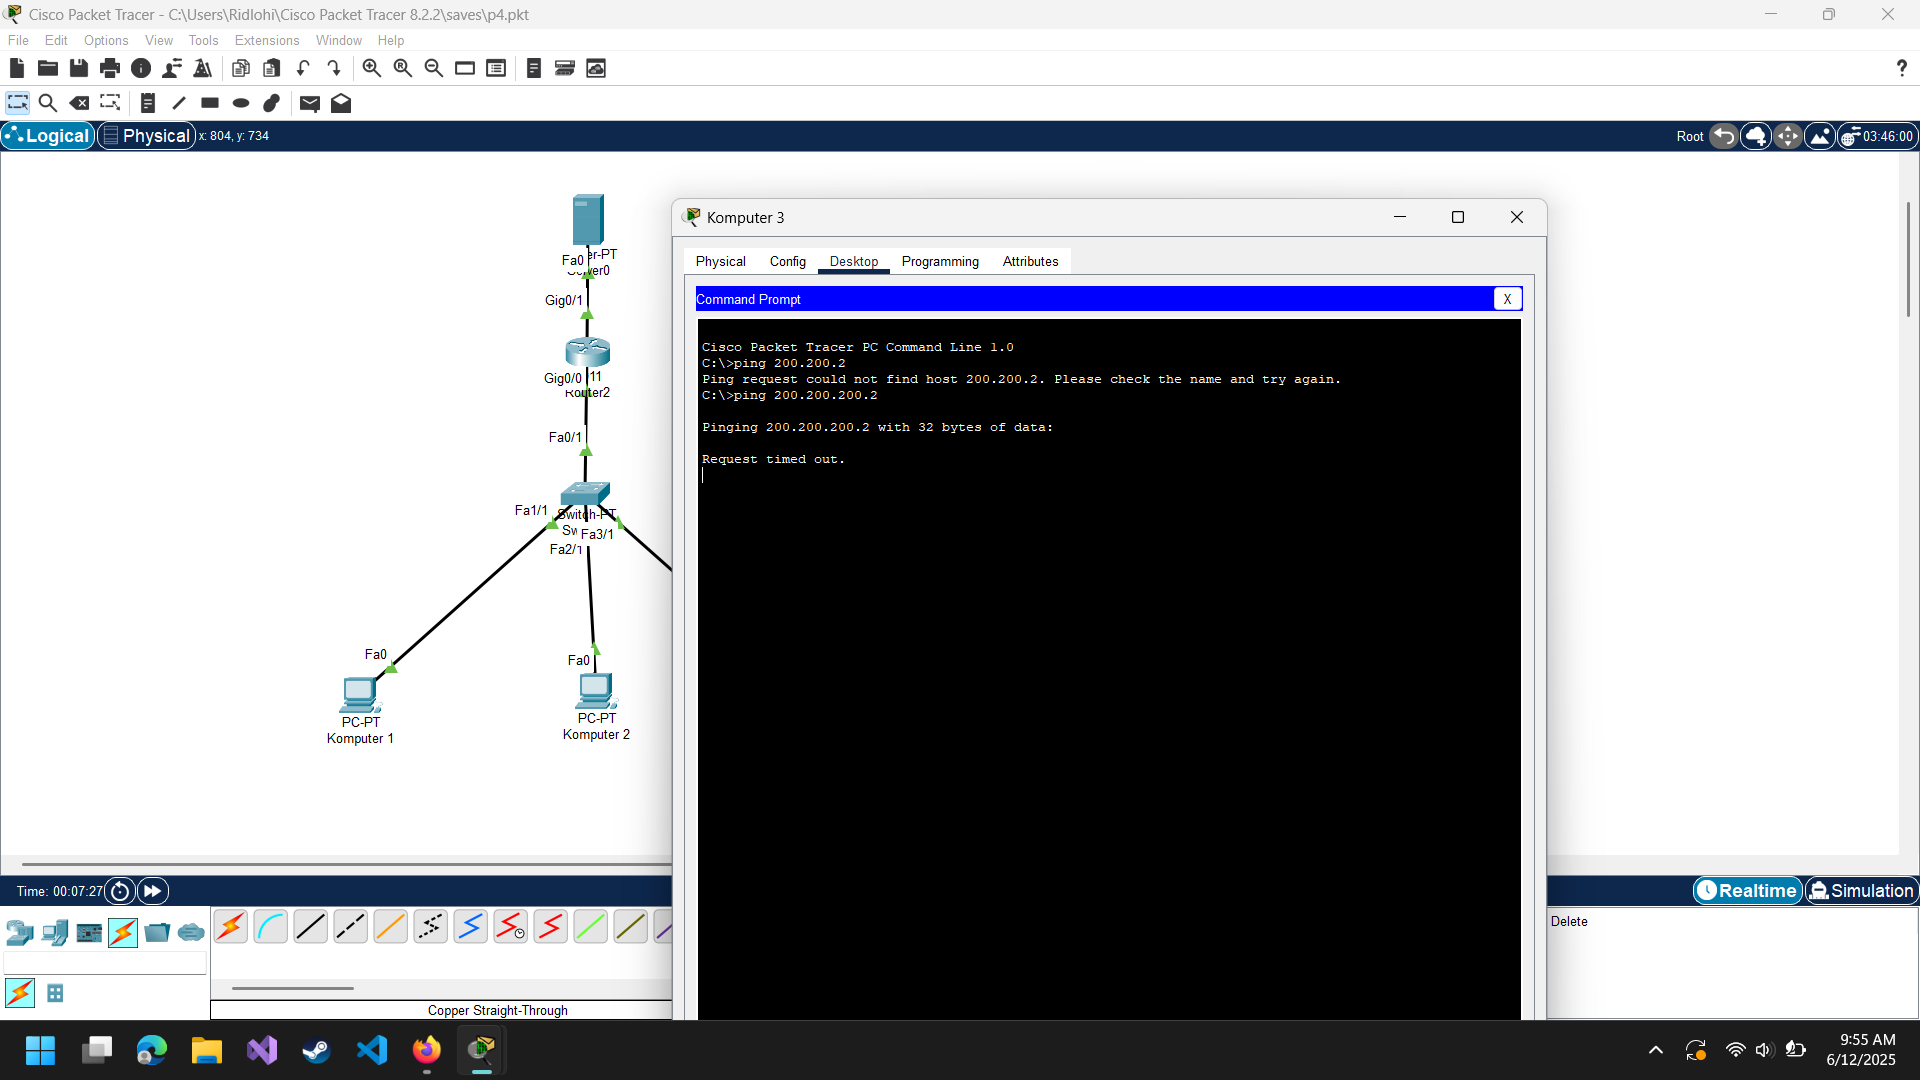
\includegraphics[width=0.5\linewidth]{pingpc3keserver.png}
        \caption{Ping PC 3 ke server}
        \label{fig:gambar}
    \end{figure}

    \begin{figure}[H]
        \centering
        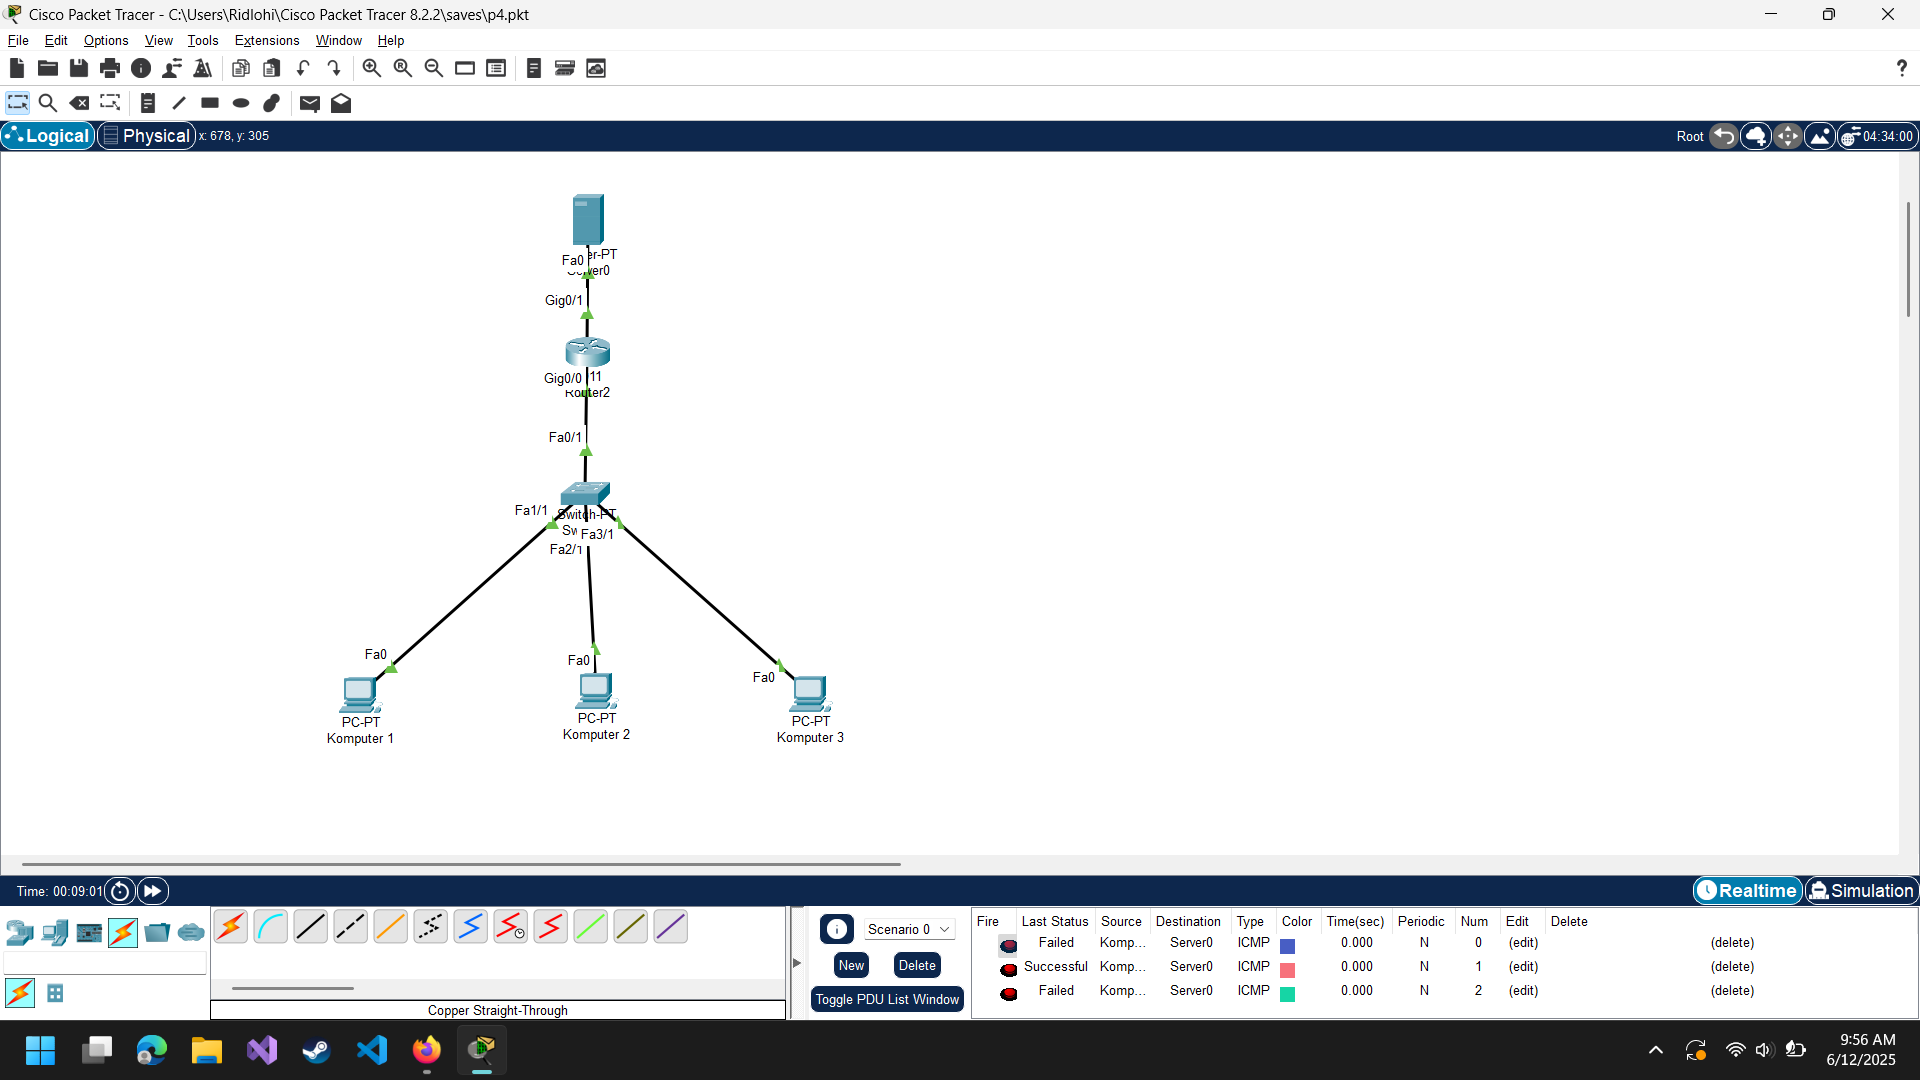
\includegraphics[width=0.5\linewidth]{pingpckeserver.png}
        \caption{Ping PC 1 dan 3 ke block ke server}
        \label{fig:gambar}
    \end{figure}
\section{Kesimpulan}
Dari hasil praktikum ini dapat disimpulkan bahwa firewall berperan penting dalam mengendalikan dan 
mengamankan lalu lintas jaringan dengan menerapkan aturan-aturan tertentu untuk mengizinkan atau 
menolak akses. Sementara itu, NAT memungkinkan efisiensi penggunaan alamat IP publik dengan 
mentranslasikan alamat IP lokal ke alamat IP publik, serta mendukung konektivitas internet bagi 
banyak perangkat dalam jaringan lokal.


\section{Lampiran}
\subsection{Dokumentasi saat praktikum}
    \begin{figure}[H]
        \centering
        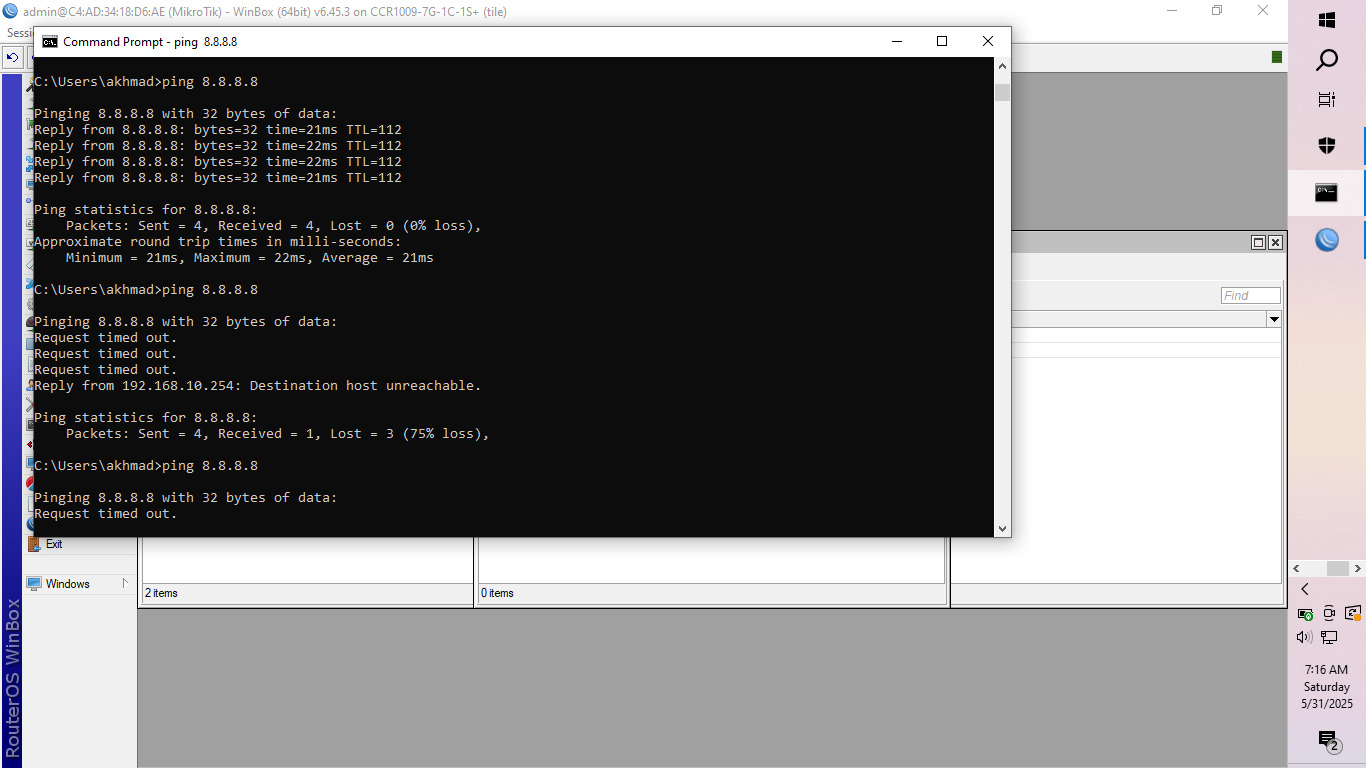
\includegraphics[width=0.5\linewidth]{gambar8a.jpeg}
        \caption{Ping dengan Firewall Aktif}
        \label{fig:ping-saat-firewall-aktif}
    \end{figure}

    \begin{figure}[H]
        \centering
        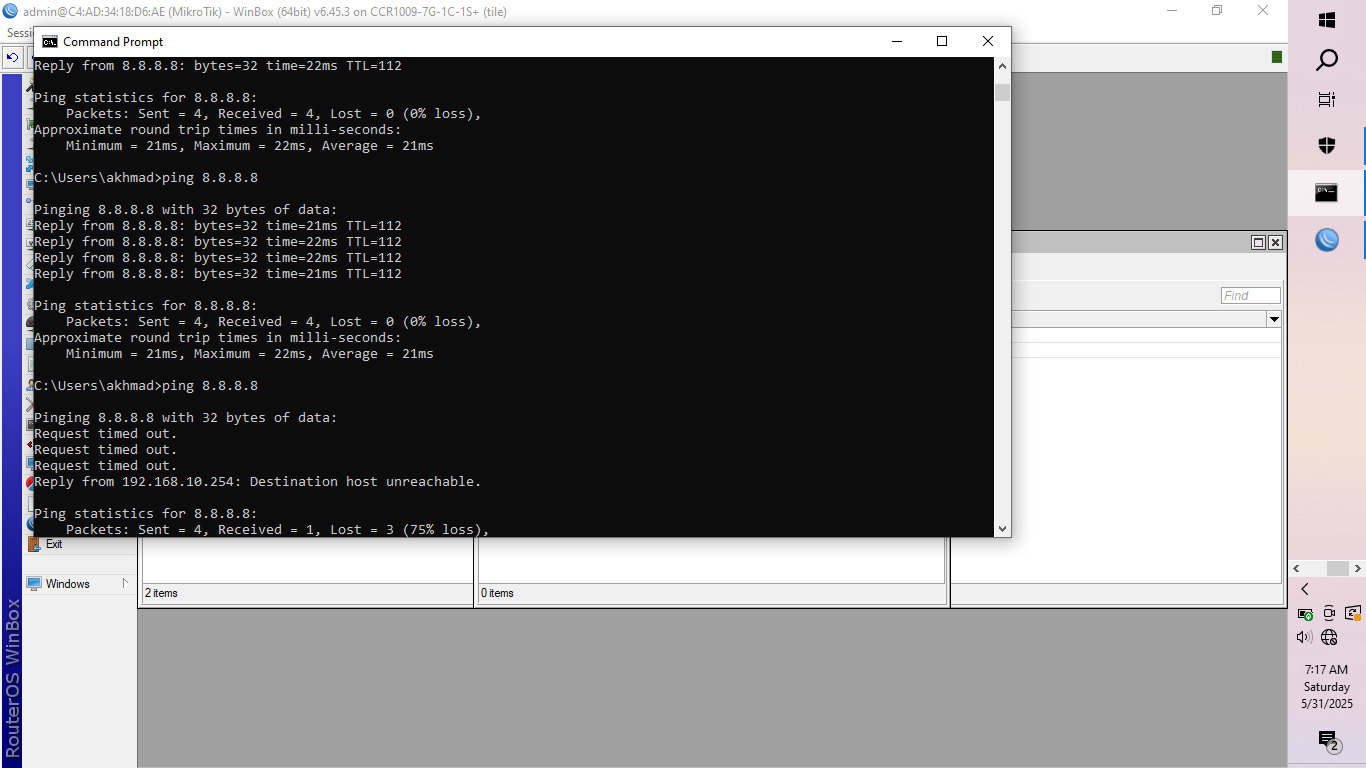
\includegraphics[width=0.5\linewidth]{gambar8b.jpeg}
        \caption{Ping dengan Firewall Tidak Aktif}
        \label{fig:ping-saat-firewall-tidak-aktif}
    \end{figure}


